\documentclass[10pt]{article}


% ==================== BASIC FORMATTING ====================
\setlength{\parindent}{0pt} % removes indents from paragraphs
\setlength{\parskip}{3pt}   % adds small space between paragraphs
% ==========================================================


% ==================== PACKAGES ====================
\usepackage{cancel} % allows striking out of text
\usepackage{xfrac} % diagonal fraction
\usepackage{float}
\usepackage{amsfonts,amssymb,amsmath,latexsym,amsthm,mathrsfs,cases} % basic [mathabx] math symbols
\usepackage{tikz}
\usetikzlibrary{arrows,automata,positioning}
\usepackage{graphicx}  % add graphics by \includegraphics
\usepackage[margin=1in]{geometry}
\usepackage{arydshln}
\usepackage{etoolbox}
\usepackage{color}
\usepackage{listings} % to add python/MATLAB code
\usepackage[final, nopatch=footnote]{microtype} % microtype
\usepackage{enumerate}
\usepackage[shortlabels]{enumitem}
\usepackage{empheq} % To use left bracket and subequations at the same time
\usepackage{titlesec}
\usepackage{subcaption}
\usepackage{caption}
\usepackage{listings} % For creating listing environments/ code boxes
\usepackage{xcolor} % Optional: for custom colors
\usepackage{pdfpages} % connect a pdf to your latex document with this
\usepackage[most]{tcolorbox} % Adds boxes into latex to emphasize different content
% =========================================================



% ==================== CODE BOXES SETUP ====================
\lstset{
    basicstyle=\footnotesize\ttfamily,
    commentstyle=\color{green!60!black},
    keywordstyle=\color{blue},
    stringstyle=\color{purple},
    breaklines=true,
    captionpos=b, % Caption position at the bottom
    % Add other desired styles
}
% =========================================================

% =========================================================
% MATLAB Code Box
% =========================================================

\definecolor{mlkeyword}{RGB}{0,0,255}
\definecolor{mlcomment}{RGB}{34,139,34}
\definecolor{mlstring}{RGB}{163,21,21}
\definecolor{mlbg}{RGB}{250,250,250}
\definecolor{mlframe}{RGB}{200,200,200}
\definecolor{mlnumbers}{RGB}{120,120,120}

\lstdefinestyle{matlabcustom}{
 language=Matlab,
 backgroundcolor=\color{mlbg},
 basicstyle=\ttfamily\small,
 keywordstyle=\color{mlkeyword}\bfseries,
 commentstyle=\color{mlcomment}\itshape,
 stringstyle=\color{mlstring},
 numberstyle=\tiny\color{mlnumbers},
 numbers=left,
 stepnumber=1,
 numbersep=8pt,
 frame=single,
 rulecolor=\color{mlframe},
 breaklines=true,
 breakatwhitespace=false,
 showstringspaces=false,
 tabsize=4,
 captionpos=b
}
% =========================================================

% ==================== LANGUAGE-SPECIFIC CODE BOXES ====================
\lstdefinestyle{pythoncustom}{
 language=Python,
 backgroundcolor=\color{mlbg},
 basicstyle=\ttfamily\small,
 keywordstyle=\color{blue}\bfseries,
 commentstyle=\color{green!60!black}\itshape,
 stringstyle=\color{purple},
 numberstyle=\tiny\color{mlnumbers},
 numbers=left,
 stepnumber=1,
 numbersep=8pt,
 frame=single,
 rulecolor=\color{mlframe},
 breaklines=true,
 showstringspaces=false,
 tabsize=4,
 captionpos=b
}

\lstdefinestyle{javacustom}{
 language=Java,
 backgroundcolor=\color{mlbg},
 basicstyle=\ttfamily\small,
 keywordstyle=\color{blue}\bfseries,
 commentstyle=\color{green!60!black}\itshape,
 stringstyle=\color{purple},
 numberstyle=\tiny\color{mlnumbers},
 numbers=left,
 stepnumber=1,
 numbersep=8pt,
 frame=single,
 rulecolor=\color{mlframe},
 breaklines=true,
 showstringspaces=false,
 tabsize=4,
 captionpos=b
}

\lstdefinestyle{cppcustom}{
 language=C++,
 backgroundcolor=\color{mlbg},
 basicstyle=\ttfamily\small,
 keywordstyle=\color{blue}\bfseries,
 commentstyle=\color{green!60!black}\itshape,
 stringstyle=\color{purple},
 numberstyle=\tiny\color{mlnumbers},
 numbers=left,
 stepnumber=1,
 numbersep=8pt,
 frame=single,
 rulecolor=\color{mlframe},
 breaklines=true,
 showstringspaces=false,
 tabsize=4,
 captionpos=b
}

\lstdefinestyle{mathematicacustom}{
 language=Mathematica,
 backgroundcolor=\color{mlbg},
 basicstyle=\ttfamily\small,
 keywordstyle=\color{blue}\bfseries,
 commentstyle=\color{green!60!black}\itshape,
 stringstyle=\color{purple},
 numberstyle=\tiny\color{mlnumbers},
 numbers=left,
 stepnumber=1,
 numbersep=8pt,
 frame=single,
 rulecolor=\color{mlframe},
 breaklines=true,
 showstringspaces=false,
 tabsize=4,
 captionpos=b
}


% ==================== TEXT BOXES SETUP ====================

\newtcolorbox{myboxb}{
  breakable,
  colback=blue!5!white,
  colframe=blue!75!black
}

\newtcolorbox{myboxr}{
 breakable,
 colback=red!5!white,
 colframe=red!75!black
}

\newtcolorbox{myboxg}{
 breakable,
 colback=green!5!white,
 colframe=green!75!black
}

% ==========================================================


% ==================== HYPERLINK SETUP ====================
\usepackage[hidelinks]{hyperref}  %% add box and hyperlinks to equation numbers
\definecolor{darkblue}{rgb}{0.0,0.0,0.3}
\hypersetup{colorlinks,breaklinks,
            linkcolor=blue,urlcolor=blue,
            anchorcolor=darkblue,citecolor=darkblue}
% =========================================================


% ==================== SECTION TITLES ====================
\titleformat{\section}[block]
  {\normalfont\large\bfseries}{Part \thesection:}{5pt}{}
\titleformat{name=\section,numberless}[block]
  {\normalfont\large\bfseries}{}{0pt}{}
% ========================================================


% ==================== CUSTOM SECTION HEADERS ====================
\newcommand{\homework}[1]{%
 \refstepcounter{section}%
 \section*{Homework \thesection: #1}%
 \addcontentsline{toc}{section}{Homework \thesection: #1}%
}

\newcommand{\exampractice}[1]{%
 \refstepcounter{section}%
 \section*{Exam Practice \thesection: #1}%
 \addcontentsline{toc}{section}{Exam Practice \thesection: #1}%
}

\newcommand{\miscnote}[1]{%
 \refstepcounter{section}%
 \section*{Additional Notes \thesection: #1}%
 \addcontentsline{toc}{section}{Additional Notes \thesection: #1}%
}

% ============================================================================


% ==================== THEOREM ENVIRONMENTS ====================
\theoremstyle{plain}
\newtheorem{theorem}{Theorem}[section]
\newtheorem{model}{Model}[section]
\newtheorem{lemma}[theorem]{Lemma}
\newtheorem{proposition}[theorem]{Proposition}
\newtheorem{corollary}[theorem]{Corollary}
\newtheorem{acknowledgement}[theorem]{Acknowledgement}
\newtheorem{algorithm}[theorem]{Algorithm}
\newtheorem{axiom}[theorem]{Axiom}
\newtheorem{case}[theorem]{Case}
\newtheorem{claim}[theorem]{Claim}
\newtheorem{conclusion}[theorem]{Conclusion}
\newtheorem{condition}[theorem]{Condition}
\newtheorem{conjecture}[theorem]{Conjecture}
\newtheorem{criterion}[theorem]{Criterion}
\newtheorem{notation}[theorem]{Notation}
\newtheorem{problem}[theorem]{Problem}
\newtheorem{summary}[theorem]{Summary}

\theoremstyle{definition}
\newtheorem{definition}{Definition}[section]
\newtheorem{result}{Result}[section]

\theoremstyle{remark}
\newtheorem{remark}{Remark}[section]
\newtheorem{bfremark}[remark]{\bf Remark}
\newtheorem{example}[remark]{Example}
\newtheorem{question}{\bf Question}[section]
\newtheorem{note}{Note}

\newtheoremstyle{exercise-style}% name
  {\topsep}% space above
  {\topsep}% space below
  {}% body font
  {}% indent amount
  {\itshape}% theorem head font
  {}% punctuation after theorem head
  {.5em}% space after theorem head
  {\thmname{#1}\thmnumber{ #2}\thmnote{ (#3)}.}% theorem head spec
\theoremstyle{exercise-style}
\newtheorem{exercise}{Exercise}[section]
\newtheorem{PCexercise}[exercise]{PC-Exercise}
% ==============================================================


% ==================== NUMBERING ====================
\numberwithin{equation}{section}
\numberwithin{theorem}{section}
\numberwithin{remark}{section}
% ===================================================


%%%%%%%% new syntax by Xiang Wan %%%%%%%%%
\newcommand{\inner}[1]{{\left\langle #1 \right\rangle}}
\newcommand{\norm}[1]{{\left\| #1 \right\|}}
\newcommand{\B}[1]{{\bf #1}}
\newcommand{\BB}[1]{{\mathbb #1}}
\newcommand{\CAL}[1]{{\mathcal #1}}
\newcommand{\inv}[1]{{#1^{-1}}}
\newcommand{\BC}{\mathbb{C}}
\newcommand{\BN}{\mathbb{N}}
\newcommand{\BP}{\mathbb{P}}
\newcommand{\BQ}{\mathbb{Q}}
\newcommand{\BR}{\mathbb{R}}
\newcommand{\BZ}{\mathbb{Z}}
\newcommand{\ds}{\displaystyle}
\newcommand{\lt}{<}
\newcommand{\normm}[2]{\left \lVert #1 \right \rVert_{#2}}
\newcommand{\HRule}[1]{\rule{\linewidth}{#1}}

%%%%%%%%%%%%%%%%%%%%%%%%%%%%%%%%%%%%%%%%%%%%%%%%%%%%%%%%%%%%%%%%%%%%%%%%%
%%%%%%%%%%%%%%%%%%%%% Do not change the lines above %%%%%%%%%%%%%%%%%%%%%
%%%%%%%%%%%%%%%%%%%%%%%%%%%%%%%%%%%%%%%%%%%%%%%%%%%%%%%%%%%%%%%%%%%%%%%%%


% ------------------------------------------------------------------------------
\title{MATH 454 - Survey of Analysis: Homework 1}
\author{Will Bales}
\date{}

\begin{document}

\maketitle

\section{Solutions}

% \begin{theorem}[Burnside's Lemma]
%     Let $G$ be a finite group acting on a finite set $X$. For each $g \in G$, let $\mathrm{Fix}(g)= \{ x \in X | g \cdot x =x \}$ be the set of elements of $X$ fixed by $g$. Then the number $k$ of orbits of $G$ on $X$ is given by:
%     \begin{align}
%         k = \frac{1}{|G|} \sum_{g \in G} |\mathrm{Fix}(g)|.
%     \end{align}
% \end{theorem}

% \begin{proof}
%     First of all we will notice that
%     \begin{align}
%         \sum_{g \in G} \sum_{x \in X} \chi(g \cdot x = x) = |\{ (g,x) \in G \times X | g \cdot x = x \}| = \sum_{x \in X} \sum_{g \in G} \chi(g \cdot x = x).
%     \end{align}
%     From this we get
%     \begin{align}
%         \sum_{g \in G}|\mathrm{Fix}(g)| = \sum_{g \in G} \sum_{x \in X} \chi (g \cdot x = x)= \sum_{x \in X} \sum_{g \in G} (g \cdot x = x) = \sum_{x \in X}|G_x|.
%     \end{align}
%     Now we see if we fix an orbit $G \cdot y$ with $x \in G \cdot y$
%     \begin{align}
%         \sum_{x \in G \cdot y} |G_x| = \sum_{x \in G \cdot y}|G_y| = |G_y| \sum_{x \in G \cdot y} 1 = |G_y||G \cdot y| = |G|
%     \end{align}
%     by the orbit stabilizer theorem. Since 
%     \begin{align}
%         \sum_{x \in X} |G_x| = \sum_{s \in G \cdot y_1}|G_x| + \cdots + \sum_{x \in G \cdot y_k}|G_x|,
%     \end{align}
%     we see
%     \begin{align}
%         \sum_{g \in G} |\mathrm{Fix}(g)| = \sum_{x \in X} |G_x| = k|G|.
%     \end{align}
%     Hence,
%     \begin{align}
%         k = \frac{1}{|G|}\sum_{g \in G} |\mathrm{Fix}(g)|
%     \end{align}
% \end{proof}

% \section{Another Part}

% \subsection{Examples of Code Boxes}

% %Below is how to insert code that you may have made in made in a paricular file

% \begin{lstlisting}[style=matlabcustom, caption={Example MATLAB code}]
% x = 1:10;
% y = x.^2;
% plot(x, y);
% \end{lstlisting}

% \begin{lstlisting}[style=pythoncustom, caption={Python example}]
%     import numpy as np
    
%     def incmatrix(genl1, genl2):
%         # comment
%         m = len(genl1)
%         n = len(genl2)
%         M = None
%         return M
% \end{lstlisting}

% \begin{lstlisting}[style=javacustom, caption={Java example}]
% class HelloWorldApp {
%     public static void main(String[] args) {
%         System.out.println("Hello World!"); // Display the string.
%     }
% }
% \end{lstlisting}

% \begin{lstlisting}[style=cppcustom, caption={C++ example}]
% #include <iostream>

% int main() {
%     std::cout << "Hello, World!" << std::endl;
%     return 0;
% }
% \end{lstlisting}

% \begin{lstlisting}[
%  style=mathematicacustom,
%  caption={Mathematica Code Taken From A File}
% ]
% (* This is a comment *)
% f[x_] := Sin[x]/x;
% Plot[f[x], {x, -10, 10}, PlotStyle -> Red]
% \end{lstlisting}

% Inserted code
% \lstinputlisting[language=Mathematica, caption={Mathematica Code Taken From A File}]{other_files/Homework_01_Grad.nb}

% \subsection{Inserting Boxes}

% We can also insert colored boxes to highlight key information

% \begin{myboxg}
%     \begin{definition}[Linear Programming]
%        We are to find the max/ min of a linear function, subject to linear constraints:
%        \begin{align}
%            & \text{max/min}(c \cdot = c_1x_1 + \cdots + c_n x_n) \\
%            \text{Subject to: } & Ax \geq b \\
%            & x \geq 0
%        \end{align}
%     \end{definition}
% \end{myboxg}

% \begin{myboxb}
%     \begin{definition}[Linear Programming]
%        We are to find the max/ min of a linear function, subject to linear constraints:
%        \begin{align}
%            & \text{max/min}(c \cdot = c_1x_1 + \cdots + c_n x_n) \\
%            \text{Subject to: } & Ax \geq b \\
%            & x \geq 0
%        \end{align}
%     \end{definition}
% \end{myboxb}

% \begin{myboxr}
%     \begin{definition}[Linear Programming]
%        We are to find the max/ min of a linear function, subject to linear constraints:
%        \begin{align}
%            & \text{max/min}(c \cdot = c_1x_1 + \cdots + c_n x_n) \\
%            \text{Subject to: } & Ax \geq b \\
%            & x \geq 0
%        \end{align}
%     \end{definition}
% \end{myboxr}

\section{Homework Assignment}

% Inserting the PDF of the Homework Assignment
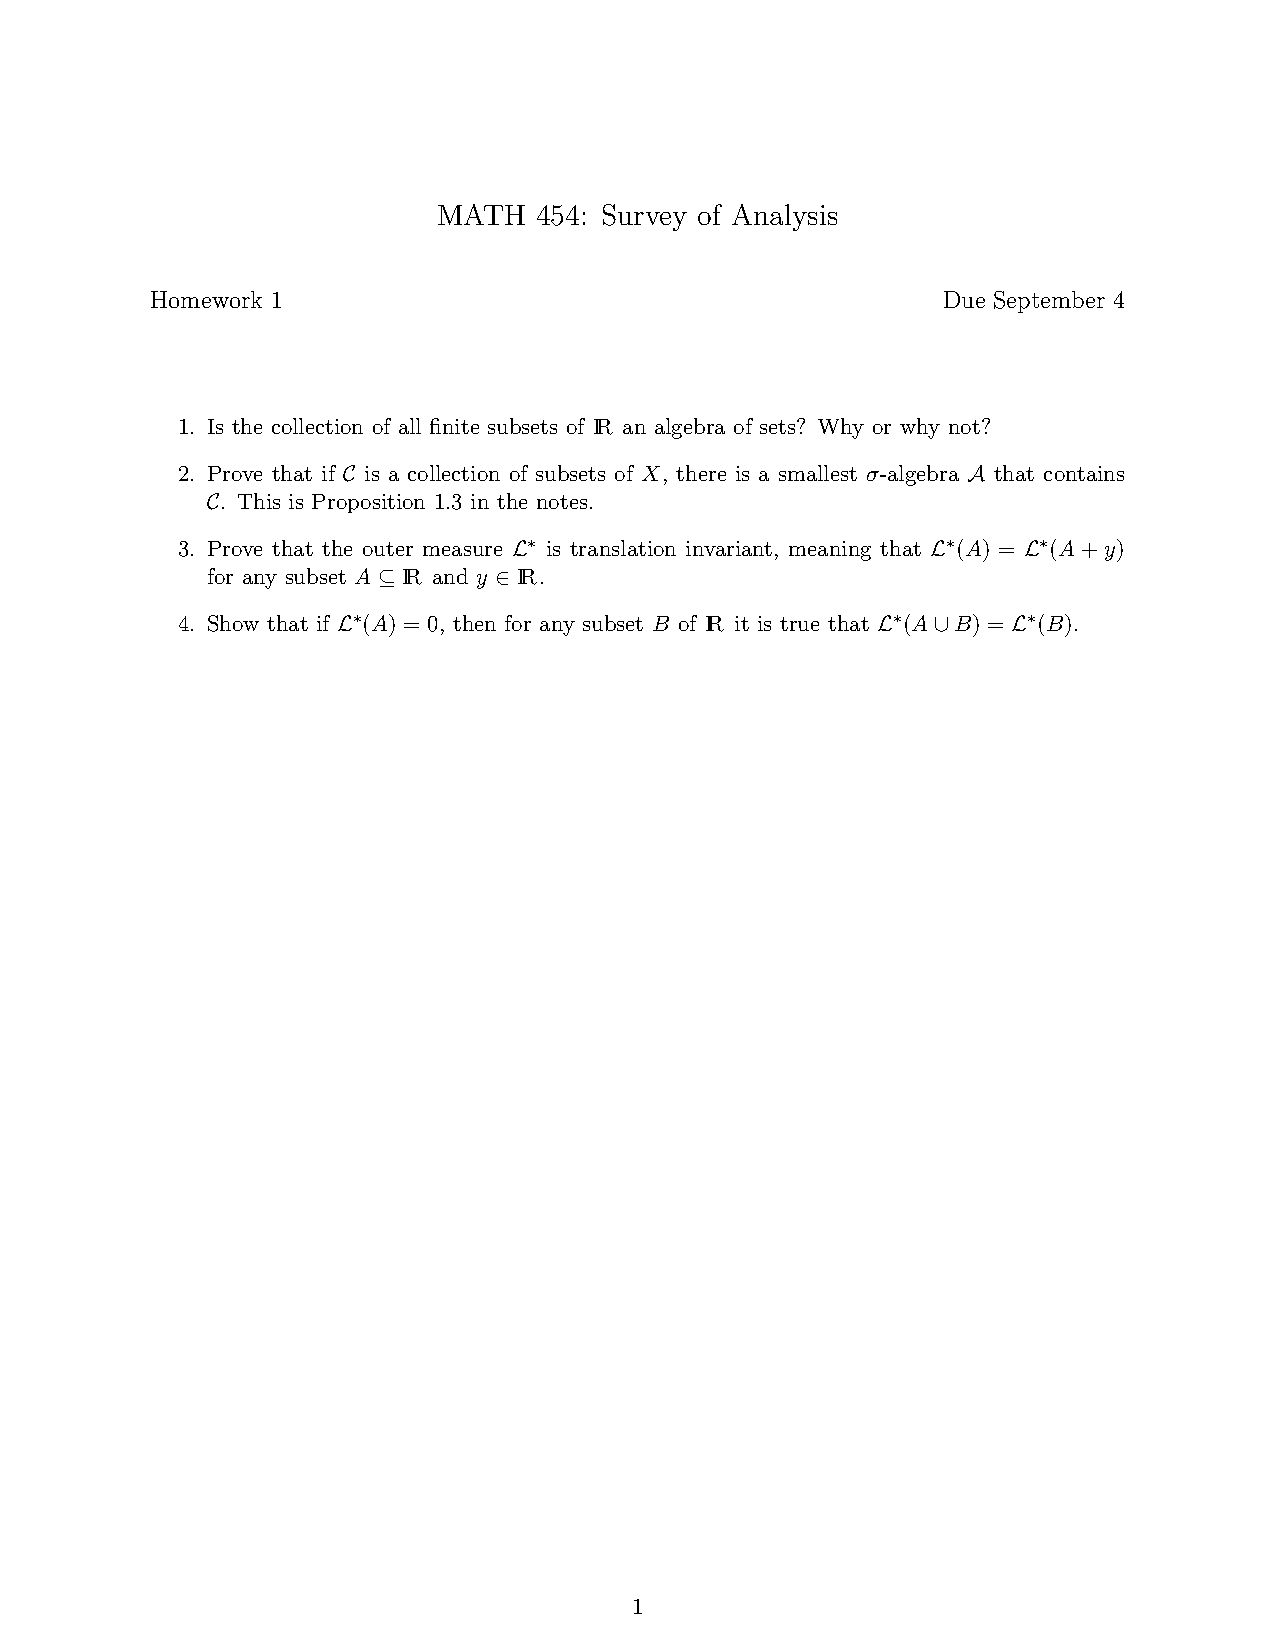
\includepdf[pages=-]{pdfs/Homework 1.pdf}

\end{document}

